
\vspace{1.5cm}


En la figura~\figref{fig:fig_p14_output_impedance} se muestra el gráfico de la impedancia en el nodo de salida en modo de regulación de corriente, el gráfico se obtuvo simulando en \textbf{SPICE} con la salida cortocircuitada a través de una fuente de tensión de señal, $V_{p}$, realizando un barrido en alterna de $0.1 \si[per-mode=symbol]{\hertz}$ a $100 \si[per-mode=symbol]{\kilo\hertz}$, con el comando \textbf{SPICE} \textit{.ac}, y luego obteniendo el cociente $\frac{V_{p}}{I\left({V_{p}}\right)}$, el resultado se exportó y se graficó en \textbf{MATLAB}, en escala semilogarítmica, su módulo y su fase, se destacó el resultado a bajas frecuencias que representa la resistencia de salida a frecuencia bajas/medias. El bajo valor obtenido para esta resistencia ($958 \si[per-mode=symbol]{\ohm}$) implica que no se trata de una buena fuente de corriente, que en el caso ideal tiene resistencia de salida $\infty$, esto se debe a la menor ganancia de lazo en modo regulación de corriente respecto al modo regulación tensión. Otra cosa que se puede observar es que al aumentar la frecuencia la impedancia disminuye, al caer la ganancia de lazo, y se torna capacitiva.




\vfill

\clearpage

\begin{figure}[H] %htb
\begin{center}
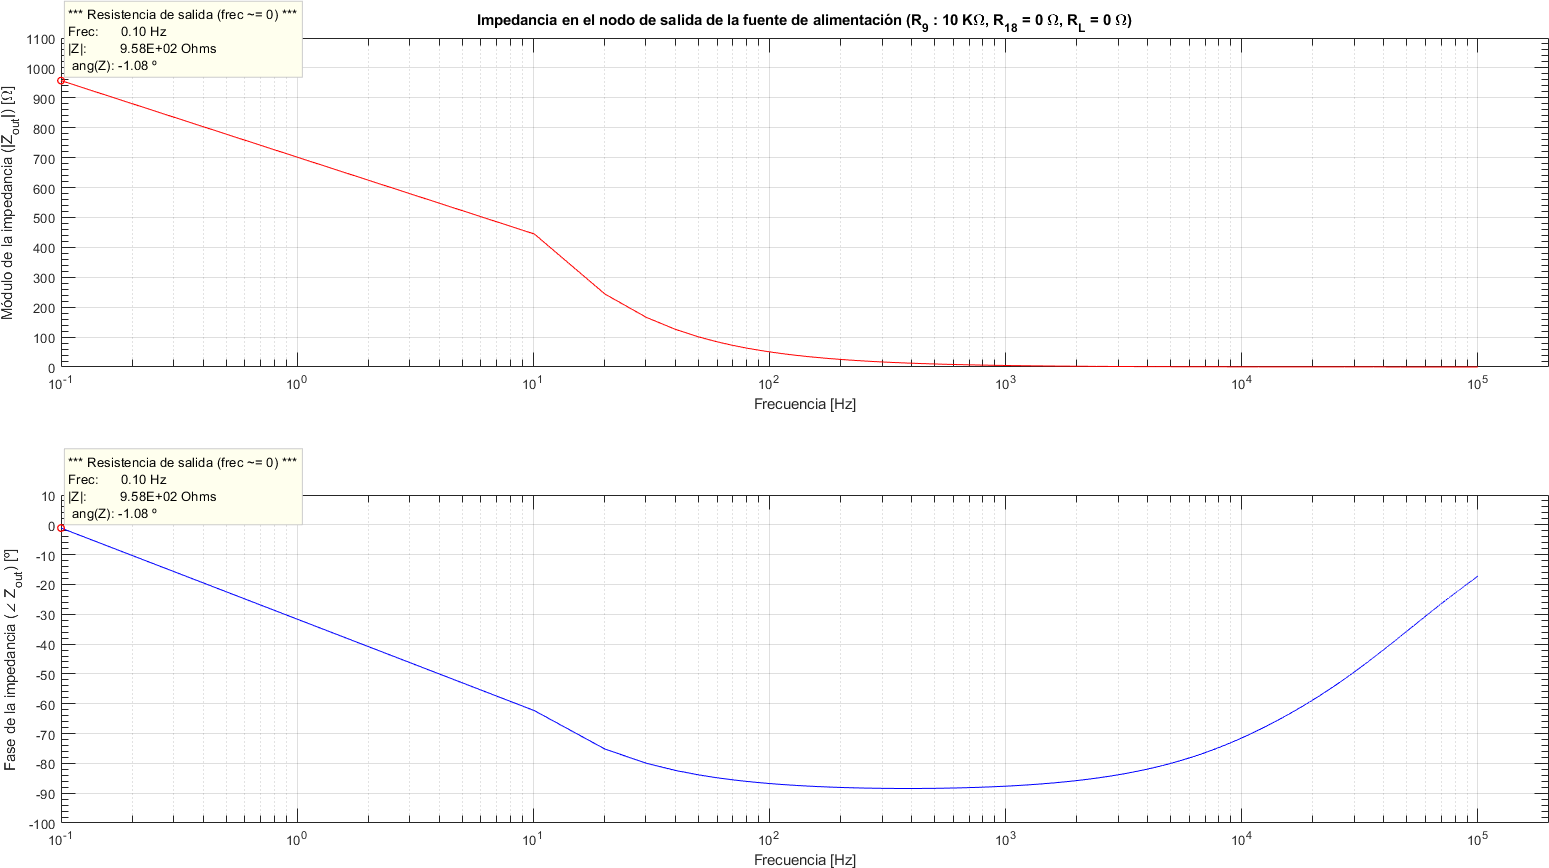
\includegraphics[width=1.2 \textwidth, angle=90]{./img/preguntas/p14.png}
\caption{\label{fig:fig_p14_output_impedance}\footnotesize{Impedancia de salida, $Z_{o}$, en función de la frecuencia, con esta variando entre $0.1 \si[per-mode=symbol]{\hertz}$ y $100 \si[per-mode=symbol]{\kilo\hertz}$.}}
\end{center}
\end{figure}



\clearpage
